%%% Local Variables:
%%% TeX-command-extra-options: "-shell-escape"
%%% mode: latex
%%% TeX-master: t
%%% End:
\documentclass{beamer}
\usepackage{caption}
\usepackage{minted}
\usepackage{tikz}
\usepackage{xcolor}
\usetikzlibrary{shapes.geometric, arrows}
\tikzstyle{startstop} = [rectangle, rounded corners, minimum width=3cm, minimum height=1cm,text centered, draw=black, fill=red!30]
\tikzstyle{io} = [trapezium, trapezium left angle=70, trapezium right angle=110, minimum width=1.5cm, minimum height=0.6cm, text centered, draw=black, fill=blue!30]
\tikzstyle{process} = [rectangle, minimum width=1.5cm, minimum height=0.5cm, text centered, draw=black, fill=orange!30]
\tikzstyle{decision} = [circle, radius=2.5cm, text centered, draw=black, fill=green!30]
\tikzstyle{arrow} = [thick,->,>=stealth]
\usepackage[labelformat=simple]{subcaption}

\usetheme{Singapore}
\title{Program Design}
%\subtitle{in Racket}
%\author{Peter Campora}
%\institute{ULL}
%\date{\today}

%This lectures introduces the fundamentals of design
\begin{document}
\begin{frame}
\titlepage
\end{frame}

\begin{frame}
  ``Lets talk about design\\
  Lets talk about programmers\\
  Lets talk about code\\
  Lets talk about bugs\\
  Lets talk about design''\\
  Celine Dion
\end{frame}

\begin{frame}
  \frametitle{Why Does Code Quality Matter?}
  \large If the program works, who cares...\\\\
  \pause
  \huge \textbf{People will read your code later!}\\\\
  \pause
  \large Ever heard of the Y2K problem? In the 20th century, digits were used to represent years...
  \begin{itemize}
  \item<4->  So, when the 21st century came, the years 1900 and 2000 would be handled identically.
  \item<5-> A ton of applications had to be updated to avoid bugs. Consider if dates were stored in poorly named int variables.
  \item<6-> Well documented code makes such refactorings easier.
  \end{itemize}
\end{frame}

\begin{frame}
  \frametitle{It Starts With a D}
  \large What is the thing that most determines the structure of a program?\\\\
  \pause
  \begin{center}
    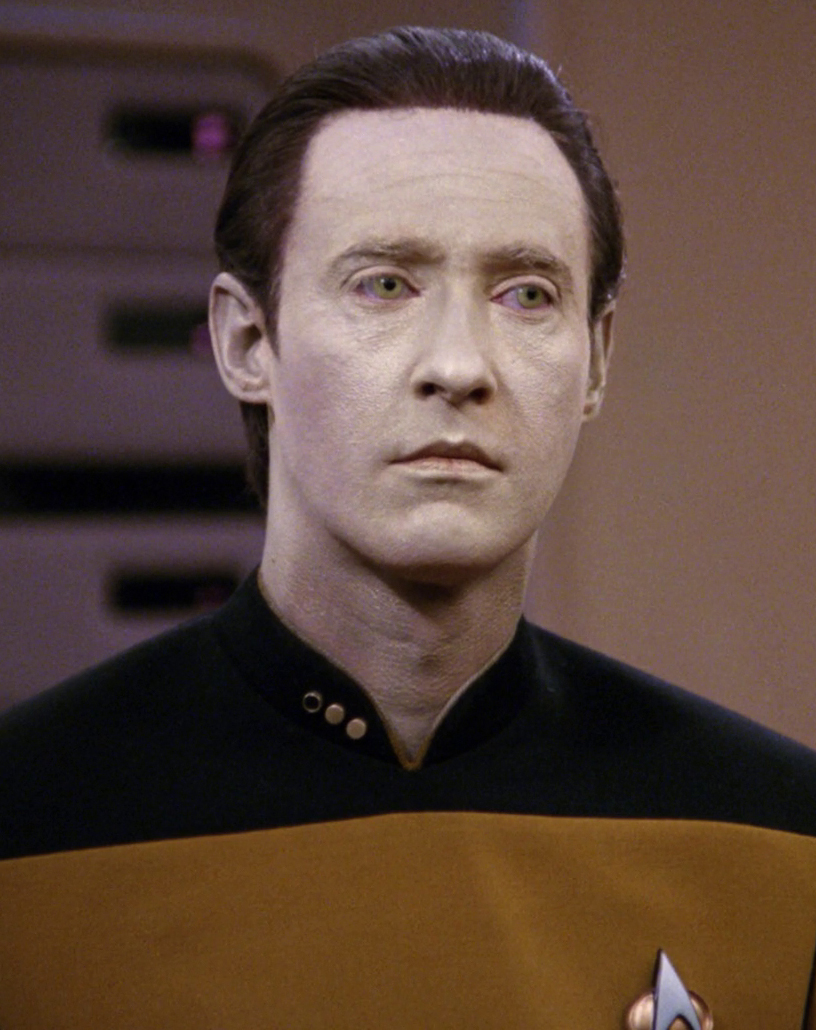
\includegraphics[width=0.4\textwidth]{images/data.jpg}
  \end{center}
\end{frame}

\begin{frame}
  \frametitle{Domains and Data}
  The two D's of software development are domains and data.
  \begin{itemize}
  \item<2-> The quantity, 5, means different things in different \emph{domains}. For a game, 4 might be the number of pixels an object should move per clock tick. For furniture website, 4 might represent the number of legs on a chair.
  \item<3-> Information in English is usually given to programmers to indicate the structure of the domain. Our job is to turn this information into \emph{data}
    representations. 
  \item<4-> After we have data representations for our domain, a program becomes a matter of data transformation.
  \item<5-> The final data produced by the program is some sort of information about our domain.
  \item<6-> If the final data is 42, this might be some height in pixels, the number of units sold, the meaning of life...etc.
  \end{itemize}
\end{frame}

\defverbatim[colored]\dataDef{
\begin{minted}{Scheme}
  ; A Temperature is a Number. 
  ; interpretation represents Celsius degrees
\end{minted}
}

\begin{frame}
  \frametitle{Data Interpretation}
  For now, we will specify the interpretation of data in comments (later we will define data types).
  \begin{itemize}
  \item<2-> We will call these data definitions. Here's an example:
  \item<3-> \dataDef
  \item<4-> This specifies that the numbers produced by our program (or function) represent Celsius degrees
  \item<5-> Such a specification rules out ``cold'' as a temperature but not -400 (which is not a real C temp)
  \item<6-> Later, we will learn to put such specifications on data, but for now our english descriptions suffice
  \end{itemize}
\end{frame}

\begin{frame}
  \frametitle{The Design Process}
  Keeping Data Interpretation in mind, let's turn to our program design process
  \begin{enumerate}
  \item<2-> Express how you wish to represent information as data. A one-line comment for specifying \emph{data interpretations} suffices.
  \item<3-> Write down a signature, a statement of purpose, and a function header.
    \begin{itemize}
    \item<4-> A \emph{signature} communicates the domain and codomain of your function. For example: \mintinline{Scheme}{; Number Number -> Number}
    \item<5-> A \emph{statement of purpose} communicates what the function produces and how it produces the answer
    \item<6-> A \emph{function header} is merely a stub definition for the function with a name, parameters, and a trivial body: \mintinline{Scheme}{(define (add x y) 0)}
    \end{itemize}    
  \end{enumerate}
\end{frame}

\begin{frame}
  \frametitle{The Design Process (cont.)}
  \begin{enumerate}
  \setcounter{enumi}{2}
  \item Create \emph{functional examples}...
\end{enumerate}
\end{frame}


\end{document}
%%% Local Variables:
%%% mode: latex
%%% TeX-master: t
%%% End:
